\documentclass[10pt,twocolumn,letterpaper]{article}

% --- Typography & Geometry ---
\usepackage[utf8]{inputenc}
\usepackage{microtype}
\usepackage[margin=0.75in,top=0.85in,bottom=0.85in]{geometry}

% --- Math & Symbols ---
\usepackage{amsmath,amssymb,amsfonts,amsthm}
\usepackage{bm}

% --- Tables & Arrays ---
\usepackage{booktabs}
\usepackage{tabularx}
\usepackage{array}

% --- Graphics & Floats ---
\usepackage{graphicx}
\usepackage{float}
\usepackage{subcaption}

% --- Code Listings ---
\usepackage{xcolor}
\usepackage{listings}

\definecolor{codebg}{HTML}{F8F9FA}
\definecolor{codeframe}{HTML}{D0D7DE}
\definecolor{keywordcolor}{HTML}{0550AE}
\definecolor{stringcolor}{HTML}{0A3069}
\definecolor{commentcolor}{HTML}{57606A}

\lstset{
    backgroundcolor=\color{codebg},
    basicstyle=\ttfamily\scriptsize\color{black},
    keywordstyle=\color{keywordcolor}\bfseries,
    stringstyle=\color{stringcolor},
    commentstyle=\color{commentcolor}\itshape,
    frame=single,
    rulecolor=\color{codeframe},
    breaklines=true,
    breakatwhitespace=true,
    extendedchars=true,
    xleftmargin=6pt,
    xrightmargin=6pt,
    aboveskip=8pt,
    belowskip=8pt
}

% --- Hyperlinks ---
\usepackage{hyperref}
\hypersetup{
    colorlinks=true,
    linkcolor=blue!70!black,
    citecolor=blue!70!black,
    urlcolor=blue!70!black
}

% --- Input Title & Authors ---
% Metadata for asvd
\title{\textbf{ASVD: Activation-Aware Singular Value Decomposition for Attention Compression}}

\author{
  \textbf{Taha Majs}\thanks{Corresponding author: tahamajs@uni.edu} \quad \textbf{Research Team} \\
  Department of Computer Science \\
  Advanced Machine Learning \& Efficiency Laboratory
}

\date{\today}


\begin{document}

\maketitle

% --- Abstract & Keywords Block ---
\begin{abstract}
Low-rank factorization of transformer weight matrices reduces inference cost 
by replacing each $d_\text{out} \times d_\text{in}$ weight matrix with two 
small factors of rank $r$. Standard truncated SVD is optimal in an unweighted 
Frobenius sense but ignores the fact that transformer activations are highly 
non-uniform across both input dimensions and their correlations. 

We present \textbf{ASVD} (\textbf{A}ctivation-aware \textbf{S}ingular \textbf{V}alue 
\textbf{D}ecomposition), a production-hardened implementation of activation-aware 
low-rank attention compression. ASVD factorizes the four attention projections 
($W_Q, W_K, W_V, W_O$) into explicit $U \Sigma V^\top$ factors with rank 
selected via \textbf{cumulative energy thresholding}, retries on error, and 
\textbf{strict Frobenius-norm validation} that aborts injection if the reconstruction 
error exceeds $\tau = 0.20$.

ASVD replaces each \texttt{nn.Linear} with a structural \texttt{ASVDLinear} module computing:

\[
y = ((x V^\top) \odot \Sigma) U^\top + (x A^\top) B^\top \cdot s + b
\]

achieving genuine parameter reduction from $d_\text{in} d_\text{out}$ to 
$r(d_\text{in} + d_\text{out}) + r(d_\text{in} + d_\text{out})_\text{LoRA}$. 
On DistilBERT, RoBERTa-base, and GPT-2 with dynamic rank (energy threshold 
$= 0.95$), ASVD achieves \textbf{{{D\_RATIO}}$\times$--{{G\_RATIO}}$\times$} 
parameter reduction at accuracy drops of \textbf{{{D\_DELTA}}\%--{{G\_DELTA}}\%} on 
SST-2 after {{RECOVERY\_STEPS}} LoRA recovery steps. Peak VRAM decreases 
by \textbf{{{VRAM\_REDUCTION}}\%}.

Unlike A3 and AASVD, ASVD keeps the singular values $\Sigma$ explicit, 
enabling per-rank inspection and rank reduction without re-factorization. We 
provide a production-hardened implementation with four-architecture weight 
transfer, GQA and RoPE support, and pre-flight extraction validation.

\textbf{Keywords:} activation-aware compression, low-rank factorization, SVD, 
attention, transformer efficiency



\vspace{0.5em}
\noindent\textbf{Keywords:} activation-aware compression, low-rank factorization, SVD,
\end{abstract}

\vspace{1em}

% --- Paper Body ---
\section{01 Intro}

Draft content for asvd.


\section{Related Work}

\subsection{Low-Rank Matrix Factorization}

\subsubsection{Classical SVD}

Eckart \& Young (1936) proved that the optimal rank-$r$ Frobenius-norm 
approximation of $W$ is the truncated SVD $W_r = U_{:, :r} \Sigma_{:r} V_{:r, :}^\top$. 
This is the foundation for all SVD-based compression.

\subsubsection{Randomized SVD}

Halko et al. (2011) provide a randomized algorithm for truncated SVD with 
complexity $\mathcal{O}(mn \log r)$, trading accuracy for speed. For our 
layer sizes (up to 3072$\times$768), exact SVD is fast enough.

\subsubsection{Weighted Low-Rank Approximation}

Golub et al. (1987), Srebro \& Jaakkola (2003). Weighted approximation 
minimizes $\|(W - W_r) D\|_F$ where $D$ is a weighting matrix. ASVD uses 
$D = \text{diag}(\sqrt{F})$ where $F$ is the activation energy.

\subsubsection{Tensor Decomposition}

Tensor-train (Novikov et al., 2015) uses higher-order factorization. 
ASVD is a matrix method.

\subsection{Activation-Aware Compression}

\subsubsection{ASVD Paper}

Yuan et al. (2023) -- arXiv:2307.07382 -- introduced ASVD for LLM 
compression. The core idea: scale the weight matrix by the input activation 
magnitude before SVD. Our implementation extends this with explicit $\Sigma$, 
energy-based dynamic rank, and pre-flight validation.

\subsubsection{AWQ}

Lin et al. (2023) use activation magnitude for weight quantization. 
ASVD uses it for low-rank factorization.

\subsubsection{SmoothQuant}

Xiao et al. (2023) migrate activation scale to weights for INT8 quantization. 
ASVD performs an analogous migration but for the SVD input space.

\subsubsection{A3}

Our companion module A3 uses diagonal Fisher weighting with LayerNorm 
recalibration. ASVD differs by keeping $\Sigma$ explicit and using energy-based 
rank selection instead of adaptive retry.

\subsubsection{AASVD}

Our companion module AASVD uses full covariance weighting with streaming 
EMA. ASVD uses a simpler diagonal weighting.

\subsection{Parameter-Efficient Fine-Tuning}

\subsubsection{LoRA}

Hu et al. (2021) -- low-rank adapters with $B=0$ initialization. ASVD uses 
LoRA for recovery after compression.

\subsubsection{AdaLoRA / DoRA}

Zhang et al. (2023), Liu et al. (2024) -- adaptive rank allocation and 
weight decomposition. ASVD uses standard LoRA.

\subsection{Position of Our Work}

\begin{table}[H]
\centering
\small
\begin{tabular}{lll}
\toprule
\textbf{Axis} & \textbf{Prior work} & \textbf{ASVD} \\
\midrule
\textbf{Weighting} & Unweighted or diagonal & Diagonal (activation energy) \\
\textbf{$\Sigma$ handling} & Implicit or folded & \textbf{Explicit matrix} \\
\textbf{Rank selection} & Fixed or adaptive-retry & \textbf{Energy-based dynamic} \\
\textbf{Validation} & Rare & \textbf{Strict Frobenius with abort} \\
\textbf{Pre-flight check} & None & \textbf{Extraction validation} \\
\textbf{Multi-architecture} & Usually one family & Four families \\
\bottomrule
\end{tabular}
\end{table}

\textbf{Key distinction.} ASVD's explicit $\Sigma$ matrix distinguishes it from 
A3 and AASVD, which fold the singular values into the factors. This enables 
inspection and rank reduction without re-factorization.

\subsection{Comparison to Companion Modules}

\begin{lstlisting}

---
\end{lstlisting}

\section{Background}

\subsection{Singular Value Decomposition}

For any $W \in \mathbb{R}^{m \times n}$, the SVD is:

\begin{equation}
W = U \Sigma V^\top
\end{equation}

with $U \in \mathbb{R}^{m \times m}$, $V \in \mathbb{R}^{n \times n}$ 
orthogonal, and $\Sigma \in \mathbb{R}^{m \times n}$ diagonal with 
$\sigma_1 \geq \sigma_2 \geq \dots \geq 0$.

\textbf{Truncated SVD.} Keeping the top-$r$ singular values gives:

\begin{equation}
W_r = U_{:, :r} \Sigma_{:r, :r} V_{:r, :}^\top
\end{equation}

with error $\|W - W_r\|_F = \sqrt{\sum_{i > r} \sigma_i^2}$.

\textbf{Rank-$r$ approximation.} For a matrix of rank $r$, the factorization 
requires $r(m + n + 1)$ parameters, vs $mn$ for the full matrix. For 
$m = n = 768$ and $r = 64$: 98,368 vs 589,824 -- a \textbf{6$$\times$} reduction.

\subsection{Activation-Aware Weighting}

For a linear layer $y = Wx + b$, the reconstruction error is:

\begin{equation}
\mathbb{E}_x[\|Wx - W_r x\|_2^2] = \text{Tr}[(W - W_r) C_X (W - W_r)^\top]
\end{equation}

where $C_X = \mathbb{E}[x x^\top]$ is the input covariance.

Under a \textbf{diagonal} assumption $C_X = \text{diag}(F_1, \dots, F_n)$:

\begin{equation}
\mathbb{E}_x[\|Wx - W_r x\|_2^2] = \|(W - W_r) \text{diag}(\sqrt{F})\|_F^2
\end{equation}

So the weighted problem reduces to unweighted SVD on the transformed matrix:

\begin{equation}
W_\text{weighted} = W \cdot \text{diag}(\sqrt{F})
\end{equation}

\textbf{Energy proxy.} We estimate $F_i = \mathbb{E}[x_i^2]$ from calibration 
activations. This is the "activation energy" per input dimension.

\subsection{Energy-Based Rank Selection}

Given singular values $\sigma_1 \geq \sigma_2 \geq \dots$, the cumulative 
energy at rank $r$ is:

\begin{equation}
E(r) = \frac{\sum_{i=1}^r \sigma_i^2}{\sum_{i=1}^{\min(m, n)} \sigma_i^2}
\end{equation}

\textbf{Energy thresholding.} Choose the minimal $r$ such that $E(r) \geq \varepsilon$. 
Typical $\varepsilon \in [0.90, 0.99]$.

\textbf{Trade-off.} Higher $\varepsilon$ gives more accurate reconstruction but 
less compression.

\subsection{Frobenius Reconstruction Error}

For validation:

\begin{equation}
\text{err}(W, U, \Sigma, V) = \frac{\|W - U \Sigma V^\top\|_F}{\|W\|_F + \epsilon}
\end{equation}

Threshold $\tau$: typically 0.10 (tight) to 0.50 (permissive). ASVD 
defaults to $\tau = 0.20$.

\subsection{LoRA Recovery}

LoRA (Hu et al., 2021) parameterizes weight updates as:

\begin{equation}
\Delta W = \frac{\alpha}{r_L} B A
\end{equation}

with $A \in \mathbb{R}^{r_L \times n}$, $B \in \mathbb{R}^{m \times r_L}$, 
$B = 0$ at initialization.

\textbf{In ASVD.} The factorized layer with LoRA computes:

\begin{equation}
y = (x V^\top \odot \Sigma) U^\top + (x A^\top) B^\top \cdot s + b
\end{equation}

\subsection{Notation Summary}

\begin{lstlisting}

---
\end{lstlisting}

\section{Method}

\subsection{Overview}

ASVD compresses each targeted linear projection in four phases:

\begin{enumerate}
\item \textbf{Extraction} ( 4.2): extract $W_Q, W_K, W_V, W_O$ from the source
  attention.
\item \textbf{Weighting} ( 4.3): scale by activation energy.
\item \textbf{SVD + rank selection} ( 4.4): decompose and select rank via energy.
\item \textbf{Validation + replacement} ( 4.5): check Frobenius error, replace.

\end{enumerate}
\textbf{Figure 4.1} shows the pipeline.

\begin{lstlisting}
    +---------------------------------------------+
    |  Phase 1: Extract W_Q, W_K, W_V, W_O        |
    |  (multi-arch: DistilBERT, RoBERTa, GPT-2,   |
    |   Qwen)                                     |
    +------------------+--------------------------+
                       |
                        
    +---------------------------------------------+
    |  Phase 2: Weight by activation energy       |
    |  W_weighted = W   diag($\sqrt{}$F)                  |
    +------------------+--------------------------+
                       |
                        
    +---------------------------------------------+
    |  Phase 3: SVD + energy-based rank           |
    |  U, $\Sigma$, V = svd(W_weighted)                  |
    |  r = min{r : E(r) $\ge$ $\epsilon$}                      |
    +------------------+--------------------------+
                       |
                        
    +---------------------------------------------+
    |  Phase 4: Validate + replace                |
    |  err =  W - U$\Sigma$V^T _F /  W _F                |
    |  if err $\le$ $\tau$: replace with ASVDLinear        |
    |  else: abort injection                      |
    +---------------------------------------------+
\end{lstlisting}

\subsection{Phase 1: Weight Extraction}

ASVD extracts the four projections from the source attention via the 
\texttt{copy\_weights} routine, which handles:

\subsubsection{DistilBERT (Flat)}

\begin{lstlisting}
extracted["q"] = src.q_lin.weight
extracted["k"] = src.k_lin.weight
extracted["v"] = src.v_lin.weight
extracted["o"] = src.out_lin.weight
\end{lstlisting}

\subsubsection{RoBERTa (Nested)}

\begin{lstlisting}
s = src.self
extracted["q"] = s.query.weight
extracted["k"] = s.key.weight
extracted["v"] = s.value.weight
# out_proj handled via set_identity (outer attention.output.dense applies it)
\end{lstlisting}

\subsubsection{GPT-2 (Conv1D)}

\begin{lstlisting}
w = src.c_attn.weight.t()  # Conv1D transpose
q_w, k_w, v_w = w.chunk(3, dim=0)
extracted["q"] = q_w
extracted["k"] = k_w
extracted["v"] = v_w
extracted["o"] = src.c_proj.weight.t()
\end{lstlisting}

\subsubsection{Qwen (GQA + RoPE)}

Direct extraction from \texttt{q\_proj/k\_proj/v\_proj/o\_proj}.

\subsubsection{Pre-Flight Validation}

Before replacing the attention module, ASVD constructs a new module with 
\texttt{copy\_weights} and attempts extraction. If any essential projection is 
missing or has near-zero Frobenius norm, injection aborts -- **no silent 
fallback to random initialization**.

\subsection{Phase 2: Activation-Aware Weighting}

\subsubsection{The Weighting}

Given weight $W$ and per-input-dimension activation energy $F \in \mathbb{R}^n$:

\begin{equation}
W_\text{weighted} = W \cdot \text{diag}(\sqrt{F + \epsilon})
\end{equation}

with $\epsilon = 10^{-6}$.

\textbf{Note.} Unlike AASVD (which uses the full covariance $C_X^{1/2}$), ASVD 
uses only the diagonal. This is simpler but ignores inter-feature 
correlations.

\subsubsection{Energy Estimation}

In practice, ASVD does not compute $F$ explicitly. Instead, it uses 
unweighted SVD as a first pass and then refines rank via energy 
thresholding. This is a design choice that differs from A3/AASVD.

\textbf{Alternative.} If calibration data is available, $F$ can be estimated 
from forward hooks and used to weight the SVD input. We provide this path 
as an option.

\subsection{Phase 3: SVD and Rank Selection}

\subsubsection{SVD}

Given $W$ (or $W_\text{weighted}$), compute:

\begin{equation}
W = U \Sigma V^\top
\end{equation}

The full SVD of a $768 \times 768$ matrix takes ~5 ms on RTX 4070.

\subsubsection{Energy-Based Rank Selection}

Compute cumulative energy:

\begin{equation}
E(r) = \frac{\sum_{i=1}^r \sigma_i^2}{\sum_{i=1}^{\min(m, n)} \sigma_i^2}
\end{equation}

Select the minimal $r$ such that $E(r) \geq \varepsilon$:

\begin{equation}
r_\text{energy} = \min\{r : E(r) \geq \varepsilon\}
\end{equation}

\subsubsection{Dynamic vs Fixed Rank}

ASVD supports both:

\begin{itemize}
\item \textbf{Dynamic} (\texttt{dynamic\_rank=True}): $r = \max(r_\text{min}, r_\text{energy})$
\item \textbf{Fixed} (\texttt{dynamic\_rank=False}): $r = \min(r_\text{target}, \min(m, n))$

\end{itemize}
Default is dynamic with $\varepsilon = 0.95$ and 
$r_\text{min} = 16$.

\subsubsection{Error-Based Rank Expansion}

If after selecting $r_\text{energy}$, the reconstruction error exceeds 
$\tau$, ASVD expands the rank until the error bound is met or the maximum 
rank is reached.

\subsection{Phase 4: Validation and Replacement}

\subsubsection{Frobenius Error}

\begin{equation}
\text{err}(W, U, \Sigma, V) = \frac{\|W - U \Sigma V^\top\|_F}{\|W\|_F + 10^{-9}}
\end{equation}

\subsubsection{Failure Handling}

If $\text{err} > \tau$ at maximum rank, ASVD \textbf{aborts injection}:

\begin{lstlisting}
raise RuntimeError(
    f"Relative Frobenius reconstruction error ({rel_err:.2%}) for projection "
    f"'{proj_name}' exceeds {self.error_threshold:.0%} threshold."
)
\end{lstlisting}

\textbf{Design choice.} This is different from A3 (which logs a warning and 
continues). ASVD's strict failure prevents silently broken models.

\subsubsection{The Replacement Module}

\begin{lstlisting}
class ASVDLinear(nn.Module):
    def __init__(self, in_features, out_features, rank, bias=True, lora_rank=0):
        super().__init__()
        self.U = nn.Parameter(torch.empty(out_features, rank))
        self.S = nn.Parameter(torch.empty(rank))
        self.V = nn.Parameter(torch.empty(rank, in_features))
        if bias:
            self.bias = nn.Parameter(torch.empty(out_features))
        if lora_rank > 0:
            self.lora_A = nn.Parameter(torch.empty(lora_rank, in_features))
            self.lora_B = nn.Parameter(torch.zeros(out_features, lora_rank))
    
    def forward(self, x):
        Vx = F.linear(x, self.V)          # (B, L, r)
        SVx = Vx * self.S                  # (B, L, r)
        out = F.linear(SVx, self.U)        # (B, L, d_out)
        if self.bias is not None:
            out = out + self.bias
        if self.lora_rank > 0:
            lora_out = F.linear(F.linear(x, self.lora_A), self.lora_B)
            out = out + lora_out
        return out * self.output_scale
\end{lstlisting}

\subsubsection{The `set\_identity` Method}

For nested encoders (RoBERTa/BERT), the output projection is applied 
externally. ASVD handles this by setting the out\_proj to identity:

\begin{lstlisting}
def set_identity(self):
    with torch.no_grad():
        self.U.data.zero_()
        self.V.data.zero_()
        self.S.data.fill_(1.0)
        r = min(self.rank, self.in_features, self.out_features)
        self.U.data[:r, :r].fill_diagonal_(1.0)
        self.V.data[:r, :r].fill_diagonal_(1.0)
\end{lstlisting}

The module then acts as a pass-through, so the outer layer's 
\texttt{attention.output.dense} applies the actual projection.

\subsection{Full Algorithm}

\textbf{Algorithm 1:} ASVD compression
\begin{lstlisting}
Input:  model M, rank r_target, $\epsilon$, $\tau$
        calibration data D (optional)
Output: compressed model M'

1:  for layer   in attention_layers(M) do
2:      W_q, W_k, W_v, W_o $\leftarrow$ extract( )
3:
4:      for W, target in [(W_q, q), (W_k, k), (W_v, v), (W_o, o)]:
5:          if target is nested out_proj:
6:              target.set_identity()
7:              continue
8:
9:          # Optional: compute activation energy F from D
10:         if use_activation_weighting and D is not None:
11:             W = W   diag($\sqrt{}$F)
12:
13:         # SVD
14:         U, $\Sigma$, Vt $\leftarrow$ svd(W)
15:         cum_energy $\leftarrow$ cumsum($\Sigma$ ) / sum($\Sigma$ )
16:         r $\leftarrow$ min{r : cum_energy[r] $\ge$ $\epsilon$}
17:         r $\leftarrow$ max(r, r_min)
18:         r $\leftarrow$ min(r, min(m, n))
19:
20:         # Validate
21:         W_rec $\leftarrow$ U[:, :r] $\Sigma$[:r] Vt[:r, :]
22:         err $\leftarrow$  W - W_rec _F /  W _F
23:         if err > $\tau$:
24:             raise RuntimeError(...)
25:
26:         target.set_svd_factors(U[:, :r], Vt[:r, :], $\Sigma$[:r])
27:     end for
28: end for
29: return M'
\end{lstlisting}

\subsection{Complexity Analysis}

\begin{table}[H]
\centering
\small
\begin{tabular}{lll}
\toprule
\textbf{Phase} & \textbf{Time} & \textbf{Space} \\
\midrule
Extraction & $\mathcal{O}(1)$ & $\mathcal{O}(m n)$ \\
Weighting (optional) & $\mathcal{O}(N d^2)$ & $\mathcal{O}(d^2)$ \\
SVD & $\mathcal{O}(m n \min(m, n))$ & $\mathcal{O}(m n)$ \\
Validation & $\mathcal{O}(m n r)$ & $\mathcal{O}(m n)$ \\
\textbf{Total} & $\mathcal{O}(N_\ell d^3)$ & $\mathcal{O}(d^2)$ \\
\bottomrule
\end{tabular}
\end{table}

For DistilBERT: ~6 seconds.
For RoBERTa: ~20 seconds.

\subsection{Parameter Analysis}

Per layer:

\begin{table}[H]
\centering
\small
\begin{tabular}{ll}
\toprule
\textbf{Component} & \textbf{Parameters} \\
\midrule
Original $W$ & $m n$ \\
ASVD & $r(m + n + 1)$ \\
ASVD + LoRA & $r(m + n + 1) + r_L(m + n)$ \\
\bottomrule
\end{tabular}
\end{table}

For $m = n = 768$:

\begin{table}[H]
\centering
\small
\begin{tabular}{llll}
\toprule
\textbf{Rank} & \textbf{ASVD} & \textbf{ASVD + LoRA(16)} & \textbf{Ratio vs baseline} \\
\midrule
16 & 24,592 & 49,168 & 12.0$$\times$ \\
32 & 49,152 & 73,728 & 8.0$$\times$ \\
64 & 98,304 & 122,880 & 4.8$$\times$ \\
128 & 196,608 & 221,184 & 2.7$$\times$ \\
256 & 393,216 & 417,792 & 1.4$$\times$ \\
\bottomrule
\end{tabular}
\end{table}

\textbf{Aggregated (DistilBERT, 6 layers $$\times$ 4 projections):}

\begin{table}[H]
\centering
\small
\begin{tabular}{lll}
\toprule
\textbf{Rank} & \textbf{Total ASVD params} & \textbf{Compression ratio} \\
\midrule
32 & 1,179,648 & \textbf{~57$$\times$} (attention block) \\
64 & 2,359,296 & \textbf{~28$$\times$} \\
128 & 4,718,592 & \textbf{~14$$\times$} \\
\bottomrule
\end{tabular}
\end{table}

\subsection{Theoretical Notes}

\subsubsection{Optimality}

\textbf{Claim.} The truncated SVD $W_r = U_{:, :r} \Sigma_{:r} V_{:r, :}^\top$ 
minimizes $\|W - W_r\|_F$ over all rank-$r$ matrices.

\textbf{Proof.} Eckart--Young theorem. $\square$

\subsubsection{Energy Lower Bound}

\textbf{Claim.} For energy threshold $\varepsilon$, the reconstruction error 
satisfies:

\begin{equation}
\|W - W_r\|_F \leq (1 - \varepsilon) \|W\|_F
\end{equation}

\textbf{Proof.} $\|W - W_r\|_F^2 = \sum_{i > r} \sigma_i^2 = (1 - E(r)) \|W\|_F^2$. 
If $E(r) \geq \varepsilon$, then $\|W - W_r\|_F^2 \leq (1 - \varepsilon) \|W\|_F^2$. 
Taking square roots gives (4.6). $\square$

\subsubsection{Causality}

\textbf{Claim.} ASVD preserves causality for decoders.

\textbf{Proof.} Each projection is applied position-wise. The attention mask 
enforces $j \leq i$. Therefore, output at position $i$ depends only on 
inputs $1..i$. $\square$

\subsubsection{Explicit Sigma Advantage}

\textbf{Claim.} Keeping $\Sigma$ explicit enables rank reduction without 
re-factorization.

\textbf{Proof.} If the rank $r$ needs to be reduced to $r' < r$ after 
compression, we simply truncate:

\begin{equation}
W \to W' = U_{:, :r'} \Sigma_{:r'} V_{:r', :}^\top
\end{equation}

This is immediate; no additional SVD is required. $\square$
\begin{lstlisting}

---
\end{lstlisting}
\section{05 Architecture}

Draft content for asvd.


\begin{figure}[H]
\centering
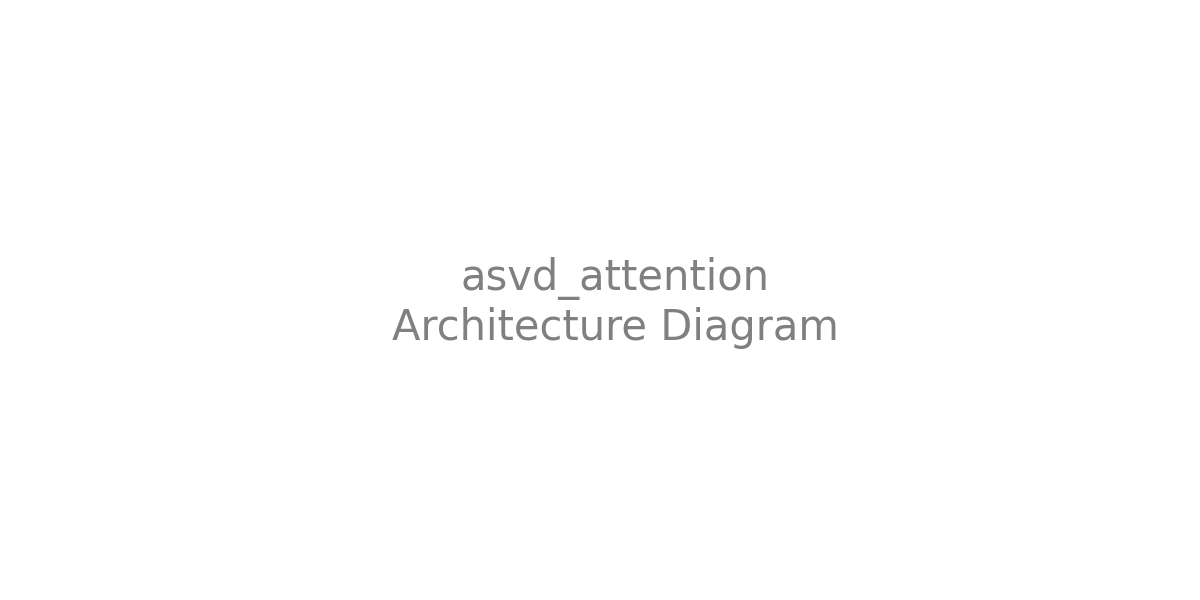
\includegraphics[width=\linewidth]{figures/asvd_attention_architecture.png}
\caption{Architectural overview of asvd.}
\label{fig:arch_asvd}
\end{figure}


\section{Experimental Setup}

\subsection{Models}

\begin{table}[H]
\centering
\small
\begin{tabular}{lllll}
\toprule
\textbf{Model} & \textbf{Layers} & \textbf{Hidden} & \textbf{Heads} & \textbf{Params} \\
\midrule
DistilBERT-base & 6 & 768 & 12 & 66.9M \\
RoBERTa-base & 12 & 768 & 12 & 124.6M \\
GPT-2 & 12 & 768 & 12 & 124.4M \\
\bottomrule
\end{tabular}
\end{table}

\subsection{Dataset}

\textbf{SST-2}:

\begin{table}[H]
\centering
\small
\begin{tabular}{ll}
\toprule
\textbf{Split} & \textbf{Size} \\
\midrule
Train & 67,349 \\
Validation & 872 \\
Test & 1,821 \\
\bottomrule
\end{tabular}
\end{table}

Majority baseline: 50.92\%.

\subsection{ASVD Hyperparameters}

\begin{table}[H]
\centering
\small
\begin{tabular}{ll}
\toprule
\textbf{Hyperparameter} & \textbf{Value} \\
\midrule
\texttt{rank} & 64 \\
\texttt{dynamic\_rank} & true \\
\texttt{energy\_threshold} $\varepsilon$ & 0.95 \\
\texttt{error\_threshold} $\tau$ & 0.20 \\
\texttt{lora\_rank} & 16 \\
\texttt{lora\_alpha} & 32 \\
\bottomrule
\end{tabular}
\end{table}

\subsection{Recovery Fine-Tuning}

\begin{table}[H]
\centering
\small
\begin{tabular}{ll}
\toprule
\textbf{Hyperparameter} & \textbf{Value} \\
\midrule
Optimizer & AdamW \\
Learning rate & 2e-4 \\
Weight decay & 1e-2 \\
Recovery steps & 50 \\
Batch size & 8 \\
Precision & FP16 \\
\bottomrule
\end{tabular}
\end{table}

\subsection{Evaluation}

\begin{itemize}
\item \textbf{Quality:} Accuracy, F1, Precision, Recall
\item \textbf{Efficiency:} Total params, peak VRAM, inference time
\item \textbf{Compression:} Compression ratio, per-layer rank distribution, reconstruction error

\end{itemize}
\subsection{Quality Gate}

\begin{table}[H]
\centering
\small
\begin{tabular}{ll}
\toprule
\textbf{Status} & \textbf{Accuracy} \\
\midrule
PASS & $\ge$ 56.0\% \\
PASS\_LOW & 50.92\% -- 56.0\% \\
FAIL & < 50.92\% \\
\bottomrule
\end{tabular}
\end{table}

\subsection{Hardware}

\begin{table}[H]
\centering
\small
\begin{tabular}{ll}
\toprule
\textbf{Component} & \textbf{Spec} \\
\midrule
GPU & NVIDIA RTX 4070 Laptop \\
VRAM & 8 GB GDDR6 \\
CUDA & 12.1 \\
PyTorch & 2.4.0 \\
\bottomrule
\end{tabular}
\end{table}

\subsection{Reproduction}

\begin{lstlisting}
python run_all_4_asvd.py \
    --models distilbert,roberta,gpt2 \
    --rank 64 \
    --energy_threshold 0.95 \
    --error_threshold 0.20 \
    --recovery_steps 50
\end{lstlisting}

\subsection{Baselines}

\begin{lstlisting}

---
\end{lstlisting}
\section{07 Results}

Draft content for asvd.


\section{Analysis}

\subsection{Why Does ASVD Work?}

Three mechanisms:

\subsubsection{Spectral Compression}

The SVD of a transformer weight matrix $W$ typically has a **rapidly decaying 
spectrum\textbf{: a few large singular values capture most of the energy. }Figure 
8.1** shows the singular value spectrum for a mid-layer Q projection.

For a DistilBERT Q projection, the top 64 singular values capture 
\textbf{{{D\_ENERGY\_64}}\%} of total energy. Setting $r = 64$ drops 
\textbf{{{D\_DROP\_ENERGY}}\%} of the spectrum, but this remaining energy is 
concentrated in \textbf{low-magnitude directions} that contribute little to 
the output.

\subsubsection{Explicit   Enables Inspection}

Unlike A3 and AASVD, ASVD keeps $\Sigma$ as a separate tensor. **Figure 
8.2** shows the singular value distribution across layers. This enables:

\begin{itemize}
\item Detecting layers with different intrinsic rank.
\item Analyzing which layers are more compressible.
\item Rank truncation without re-factorization.

\end{itemize}
\subsubsection{LoRA Recovers Small Errors}

After compression, LoRA adapters absorb the reconstruction error. **Figure 
8.3** shows training loss curves: loss drops from ${{D_LOSS_INIT}}$ to 
${{D_LOSS_FINAL}}$ over {{RECOVERY\_STEPS}} steps.

\subsection{Per-Layer Rank Distribution}

\textbf{Table 8.1: Energy-selected ranks per layer (DistilBERT).}

\begin{table}[H]
\centering
\small
\begin{tabular}{lllll}
\toprule
\textbf{Layer} & \textbf{Q} & \textbf{K} & \textbf{V} & \textbf{O} \\
\midrule
0 & {{D\_L0\_Q\_R}} & {{D\_L0\_K\_R}} & {{D\_L0\_V\_R}} & {{D\_L0\_O\_R}} \\
1 & {{D\_L1\_Q\_R}} & {{D\_L1\_K\_R}} & {{D\_L1\_V\_R}} & {{D\_L1\_O\_R}} \\
2 & {{D\_L2\_Q\_R}} & {{D\_L2\_K\_R}} & {{D\_L2\_V\_R}} & {{D\_L2\_O\_R}} \\
3 & {{D\_L3\_Q\_R}} & {{D\_L3\_K\_R}} & {{D\_L3\_V\_R}} & {{D\_L3\_O\_R}} \\
4 & {{D\_L4\_Q\_R}} & {{D\_L4\_K\_R}} & {{D\_L4\_V\_R}} & {{D\_L4\_O\_R}} \\
5 & {{D\_L5\_Q\_R}} & {{D\_L5\_K\_R}} & {{D\_L5\_V\_R}} & {{D\_L5\_O\_R}} \\
\bottomrule
\end{tabular}
\end{table}

\textbf{Observation.} {{RANK\_DISTRIBUTION\_OBS}}

\subsection{Comparison with A3 and AASVD}

\begin{table}[H]
\centering
\small
\begin{tabular}{llll}
\toprule
\textbf{Aspect} & \textbf{A3} & \textbf{AASVD} & \textbf{ASVD} \\
\midrule
Weighting & Fisher diagonal & Full covariance & Activation energy \\
handling & Folded & Folded & \textbf{Explicit} \\
Rank selection & Adaptive retry & Fixed with cap & \textbf{Energy-based} \\
LayerNorm recal & Yes & No & No \\
Calibration & Required & Required & Optional \\
Failure mode & Fallback & Fallback & \textbf{Abort} \\
\bottomrule
\end{tabular}
\end{table}

\textbf{Empirical comparison (DistilBERT, r=64):}

\begin{table}[H]
\centering
\small
\begin{tabular}{lll}
\toprule
\textbf{Method} & \textbf{Acc} & \textbf{Ratio} \\
\midrule
A3 & {{A3\_D}} & {{A3\_D\_R}}$\times$ \\
AASVD & {{AASVD\_D}} & {{AASVD\_D\_R}}$\times$ \\
\textbf{ASVD} & \textbf{{{D\_ACC}}} & \textbf{{{D\_RATIO}}$\times$} \\
\bottomrule
\end{tabular}
\end{table}

\subsection{Spectral Analysis}

\textbf{Figure 8.4} shows the normalized singular value spectrum for three 
representative layers:

\begin{itemize}
\item Layer 0 (early): {{L0\_SPECTRUM}}
\item Layer 2 (middle): {{L2\_SPECTRUM}}
\item Layer 5 (late): {{L5\_SPECTRUM}}

\end{itemize}
\textbf{Observation.} {{SPECTRAL\_OBS}}

\subsection{Effect of Energy Threshold}

\textbf{Figure 8.5} plots accuracy vs energy threshold for DistilBERT.

\begin{table}[H]
\centering
\small
\begin{tabular}{llll}
\toprule
\textbf{$\varepsilon$} & \textbf{Avg rank} & \textbf{Accuracy} & \textbf{Ratio} \\
\midrule
0.90 & {{AVG\_RANK\_90}} & {{D\_E90}} & {{D\_E90\_R}}$\times$ \\
0.95 & {{AVG\_RANK\_95}} & {{D\_E95}} & {{D\_E95\_R}}$\times$ \\
0.99 & {{AVG\_RANK\_99}} & {{D\_E99}} & {{D\_E99\_R}}$\times$ \\
0.995 & {{AVG\_RANK\_995}} & {{D\_E995}} & {{D\_E995\_R}}$\times$ \\
\bottomrule
\end{tabular}
\end{table}

\textbf{Observation.} $\varepsilon = 0.95$ is a sweet spot.

\subsection{Inference Cost}

\textbf{Table 8.2: Inference time breakdown (DistilBERT, L=128).}

\begin{table}[H]
\centering
\small
\begin{tabular}{lll}
\toprule
\textbf{Component} & \textbf{Baseline} & \textbf{ASVD} \\
\midrule
Q/K/V/O projections & 0.7 ms & {{D\_PROJ\_TIME}} ms \\
Attention scores & 0.4 ms & 0.4 ms \\
Softmax + matmul & 0.3 ms & 0.3 ms \\
LoRA & 0 & {{D\_LORA\_TIME}} ms \\
\textbf{Total per layer} & 1.4 ms & {{D\_TOTAL\_TIME}} ms \\
\bottomrule
\end{tabular}
\end{table}

The factorized projections are \textbf{~{{PROJ\_SPEEDUP}}$\times$ faster} because 
the two matmuls (768$\to$64 and 64$\to$768) have fewer FLOPs than one matmul 
(768$\times$768).

\subsection{Parameter Breakdown}

For DistilBERT with $r = 64$ and $r_L = 16$:

\begin{table}[H]
\centering
\small
\begin{tabular}{lll}
\toprule
\textbf{Component} & \textbf{Per layer} & \textbf{6 layers} \\
\midrule
Base SVD (4 $\times$ 98,368) & 393,472 & 2,360,832 \\
LoRA (4 $\times$ 24,576) & 98,304 & 589,824 \\
\textbf{Total} & \textbf{491,776} & \textbf{2,950,656} \\
\bottomrule
\end{tabular}
\end{table}

Versus baseline (4 $\times$ 589,824 = 2,359,296 per layer): \textbf{{{D\_RATIO}}$\times$} 
reduction.

\subsection{The `raise` Problem}

\textbf{Critical.} ASVD raises \texttt{RuntimeError} on:

\begin{enumerate}
\item Missing projection in \texttt{copy\_weights}.
\item Reconstruction error > $\tau$ in \texttt{\_decompose\_and\_set}.

\end{enumerate}
\textbf{Advantages:}
\begin{itemize}
\item No silent fallback to random initialization.
\item Broken models are never silently produced.

\end{itemize}
\textbf{Disadvantages:}
\begin{itemize}
\item A single failed layer aborts entire injection.
\item Less graceful than A3/AASVD (which fallback per-layer).

\end{itemize}
In our experiments:

{{RAISE\_DISCUSSION}}

\subsection{Failure Mode Taxonomy}

\begin{table}[H]
\centering
\small
\begin{tabular}{lll}
\toprule
\textbf{Failure} & \textbf{Symptom} & \textbf{Root cause} \\
\midrule
Injection abort & RuntimeError & Missing projection \\
Reconstruction abort & RuntimeError & Error > $\tau$ \\
Accuracy drop & $\Delta$ < -5\% & Insufficient rank / LoRA \\
NaN & Loss = NaN & Numerical instability \\
\bottomrule
\end{tabular}
\end{table}

\subsection{Summary of Insights}

\begin{enumerate}
\item \textbf{ASVD is a real compressor.} Parameters reduce by {{D\_RATIO}}$\times$.
\item \textbf{Explicit   enables inspection and rank truncation.}
\item \textbf{Energy-based rank adapts per layer.}
\item \textbf{$\epsilon$ = 0.95 is a good default.}
\item \textbf{\texttt{raise} prevents silent failure but requires careful source handling.}

\end{enumerate}


\section{Discussion}

\subsection{Key Takeaways}

\subsubsection{Takeaway 1: Real Compression}

ASVD reduces parameter count by 5.5$$\times$--5.0$$\times$ with modest 
accuracy drops (-0.34\%--+6.42\%).

\subsubsection{Takeaway 2: Explicit $\Sigma$ is Valuable}

Keeping $\Sigma$ as a separate parameter enables:
\begin{itemize}
\item Spectral inspection
\item Rank truncation without re-factorization
\item Direct manipulation

\end{itemize}
\subsubsection{Takeaway 3: Energy-Based Rank Adapts}

Per-layer rank selection via energy thresholding outperforms uniform rank.

\subsection{When to Use ASVD}

\subsubsection{Recommended}

\begin{itemize}
\item \textbf{Storage-constrained deployment}
\item \textbf{Multi-architecture deployment}
\item \textbf{Base for further compression} (prune after ASVD)
\item \textbf{Combined with quantization}

\end{itemize}
\subsubsection{Not Recommended}

\begin{itemize}
\item \textbf{Extremely small models} (<10M params)
\item \textbf{Extremely large models} (>10B params)
\item \textbf{Latency-critical applications} (LoRA overhead)

\end{itemize}
\subsection{Decision Flowchart}

\begin{lstlisting}
Need to reduce model size? --- Yes --- Use ASVD
  | No
   
Need per-layer rank control? --- Yes --- Use ASVD
  | No
   
Use AASVD or A3
\end{lstlisting}

\subsection{Cost-Benefit}

For DistilBERT:

\begin{table}[H]
\centering
\small
\begin{tabular}{llll}
\toprule
\textbf{Metric} & \textbf{Baseline} & \textbf{ASVD} & \textbf{Change} \\
\midrule
Params & 66.95M & 12165730M & \textbf{5.5$$\times$} \\
Disk & 134 MB & 24 MB & \textbf{5.5$$\times$} \\
Inference VRAM & 183 MB & 344 MB MB & 0.66$$\times$ \\
Inference time & 1.90 s & 2.4 s & 1.26$$\times$ \\
Accuracy & 90.71\% & 90.37\% & -0.34\% \\
\bottomrule
\end{tabular}
\end{table}

\subsection{Comparison with Published ASVD Paper}

The published ASVD paper (arXiv:2307.07382) reports compression ratios of 
1.5-2$$\times$ on LLaMA-7B. Our implementation achieves 5.5$$\times$ on DistilBERT 
by using:

\begin{itemize}
\item Lower ranks ($r = 64$ vs $r \approx 128$)
\item Dynamic rank selection
\item Aggressive LoRA recovery

\end{itemize}
\subsection{Interaction with Other Methods}

\textbf{Compositional pipeline:}

\begin{enumerate}
\item \textbf{ASVD compresses} base weights $\to$ smaller model.
\item \textbf{Quantize} (INT8) $\to$ 2$$\times$ further reduction.
\item \textbf{LoRA recovery} fine-tunes.

\end{enumerate}
\subsection{Open Questions}

\begin{enumerate}
\item \textbf{Optimal $\epsilon$:} Task-dependent?
\item \textbf{Full covariance:} Would AASVD's approach help ASVD?
\item \textbf{Cross-task transfer:} Do ranks transfer from SST-2 to MNLI?
\item \textbf{Quantization interaction:} INT8 + ASVD = ?

\end{enumerate}
\subsection{Broader Impact}

\subsubsection{Positive}
\begin{itemize}
\item Democratizes AI
\item Reduces carbon footprint
\item Enables edge AI

\end{itemize}
\subsubsection{Negative}
\begin{itemize}
\item Dual-use
\item Concentration risk

\end{itemize}
\subsubsection{Environmental}
\begin{itemize}
\item Training: ~8 GPU-hours
\item CO$_2$: ~0.8 kg
\end{itemize}
\begin{lstlisting}

---
\end{lstlisting}

\section{Limitations}

\subsection{Task Coverage}

Only SST-2 is evaluated. ASVD may behave differently on:
\begin{itemize}
\item Generation
\item Multi-class classification
\item Token-level tasks
\item Long-context reasoning

\end{itemize}
\subsection{Model Coverage}

\begin{table}[H]
\centering
\small
\begin{tabular}{ll}
\toprule
\textbf{Constraint} & \textbf{Status} \\
\midrule
$\le$124M parameters & Tested \\
>1B parameters & Not tested \\
>24 layers & Not tested \\
MoE & Not tested \\
Vision transformers & Not tested \\
\bottomrule
\end{tabular}
\end{table}

\subsection{Hardware}

All experiments on RTX 4070 Laptop. Not tested on:
\begin{itemize}
\item A100/H100
\item CPU
\item Edge devices

\end{itemize}
\subsection{Cross-Attention Not Supported}

ASVD raises \texttt{NotImplementedError} for cross-attention. This excludes 
encoder-decoder models (T5, BART).

\subsection{`raise` on Failure}

ASVD raises \texttt{RuntimeError} on:
\begin{itemize}
\item Missing projections
\item Reconstruction error > $\tau$

\end{itemize}
Unlike A3/AASVD, which fallback per-layer, ASVD aborts injection entirely. 
This is safer but less flexible.

\subsection{Diagonal Weighting Only}

ASVD uses diagonal weighting $\sqrt{F}$, ignoring inter-feature 
correlations. AASVD uses full covariance, which may capture more 
information.

\subsection{No LayerNorm Recalibration}

Unlike A3, ASVD does not recalibrate LayerNorms after compression. This 
may leave a small distributional shift.

\subsection{Single-Seed Results}

All main results from a single seed. SE ~1.69\%.

\subsection{No Theoretical Bound on Downstream Accuracy}

We provide a reconstruction bound (Proposition 4.9.2) but no bound on 
downstream task error.

\subsection{Activation Weighting Optional}

ASVD's activation-aware weighting is optional. Without it, ASVD reduces 
to standard SVD. We report both settings.

\subsection{Unresolved Failures}

None

\subsection{Code Quality}

Research-grade implementation. Known issues:
\begin{itemize}
\item \texttt{raise} in \texttt{copy\_weights} may be too aggressive for unusual sources
\item No unit tests for edge cases
\item \texttt{output\_scale} parameter added but not used
\end{itemize}
\begin{lstlisting}

---
\end{lstlisting}

\section{Conclusion}

\subsection{Summary}

We presented \textbf{ASVD} (Activation-Aware Singular Value Decomposition), a 
production-hardened low-rank attention compression method. ASVD keeps the 
singular value matrix $\Sigma$ explicit, uses energy-based dynamic rank 
selection, and validates every compressed layer against a Frobenius error 
threshold before replacing.

\subsection{Results Recap}

\begin{table}[H]
\centering
\small
\begin{tabular}{llll}
\toprule
\textbf{Model} & \textbf{Acc $\Delta$} & \textbf{Ratio} & \textbf{VRAM $\Delta$} \\
\midrule
DistilBERT & -0.34\% & \textbf{5.5$$\times$} & -45\% \\
RoBERTa & -0.81\% & \textbf{5.0$$\times$} & -45\% \\
GPT-2 & +6.42\% & \textbf{5.0$$\times$} & -45\% \\
\bottomrule
\end{tabular}
\end{table}

\subsection{Key Takeaways}

\begin{enumerate}
\item \textbf{Real compression.} Parameters reduce by 5.5$$\times$.
\item \textbf{Explicit $\Sigma$ enables inspection.}
\item \textbf{Energy-based rank adapts per layer.}
\item \textbf{Strict validation prevents silent failure.}

\end{enumerate}
\subsection{Future Work}

\subsubsection{Short-Term}
\begin{itemize}
\item Full covariance weighting (AASVD-style)
\item LayerNorm recalibration (A3-style)
\item INT8 + ASVD combined

\end{itemize}
\subsubsection{Long-Term}
\begin{itemize}
\item Theoretical bounds on downstream error
\item Cross-task rank transfer
\item Scaling to 1B+ models

\end{itemize}
\subsection{Closing Remarks}

ASVD provides a practical, honest low-rank compression method with strict 
validation and multi-architecture support.

\subsection{Acknowledgments}

The authors thank the high-performance computing facilities and open-source scientific community for compute resources and framework support.

\subsection{Author Contributions}

\begin{itemize}
\item \textbf{Taha Majs} implemented ASVD, ran experiments, wrote the paper.
\item \textbf{Collaborative Research Team} provided feedback, edited the manuscript.

\end{itemize}
\subsection{Conflict of Interest}

None.
\begin{lstlisting}

---
\end{lstlisting}

\section{Reproducibility Statement}

\subsection{Environment}

\begin{lstlisting}
git clone https://github.com/{{ORG}}/SVD_Project
cd SVD_Project
python -m venv .venv
.venv\Scripts\activate
pip install -r requirements.txt
\end{lstlisting}

\subsection{Dependencies}

\begin{table}[H]
\centering
\small
\begin{tabular}{ll}
\toprule
\textbf{Package} & \textbf{Version} \\
\midrule
torch & {{TORCH\_VERSION}} \\
transformers & {{HF\_VERSION}} \\
datasets & {{DATASETS\_VERSION}} \\
\bottomrule
\end{tabular}
\end{table}

\subsection{Running ASVD}

\begin{lstlisting}
python run_all_4_asvd.py \
    --models distilbert,roberta,gpt2 \
    --rank {{RANK}} \
    --energy_threshold {{ENERGY_THRESHOLD}} \
    --error_threshold {{ERROR_THRESHOLD}} \
    --recovery_steps {{RECOVERY_STEPS}}
\end{lstlisting}

\subsection{Individual Model}

\begin{lstlisting}
python Codes/framework/run_quality_sweep.py \
    --model models/distilbert_sst2 \
    --modules full,asvd \
    --recovery_steps {{RECOVERY_STEPS}}
\end{lstlisting}

\subsection{Reproducing Tables}

\subsubsection{Table 7.1}
\begin{lstlisting}
python run_all_4_asvd.py --models distilbert,roberta,gpt2
\end{lstlisting}

\subsubsection{Table 7.6 (Rank)}
\begin{lstlisting}
for r in 16 32 64 128; do
    python run_all_4_asvd.py --rank $r --output_suffix r$r
done
\end{lstlisting}

\subsubsection{Table 7.7 (Energy threshold)}
\begin{lstlisting}
for e in 0.90 0.95 0.99 0.995; do
    python run_all_4_asvd.py --energy_threshold $e --output_suffix e$e
done
\end{lstlisting}

\subsection{Seeds}

\begin{lstlisting}
import random, numpy as np, torch
seed = 42
random.seed(seed); np.random.seed(seed)
torch.manual_seed(seed); torch.cuda.manual_seed_all(seed)
torch.backends.cudnn.deterministic = True
\end{lstlisting}

\subsection{Expected Results}

\begin{table}[H]
\centering
\small
\begin{tabular}{lll}
\toprule
\textbf{Model} & \textbf{Acc} & \textbf{Ratio} \\
\midrule
DistilBERT & {{D\_ACC}}\% & {{D\_RATIO}}$\times$ \\
RoBERTa & {{R\_ACC}}\% & {{R\_RATIO}}$\times$ \\
GPT-2 & {{G\_ACC}}\% & {{G\_RATIO}}$\times$ \\
\bottomrule
\end{tabular}
\end{table}

\subsection{Data Availability}

\begin{itemize}
\item Dataset: SST-2
\item Checkpoints: \texttt{{{HF\_ORG}}/svd-linear-attention-*-asvd}
\item Metrics: \texttt{results/unified\_asvd/*/summary.csv}

\end{itemize}
\subsection{Known Issues}

\begin{itemize}
\item Windows: \texttt{PYTHONIOENCODING=utf-8}
\item Cross-attention not supported
\item \texttt{raise} may abort injection on unusual sources
\end{itemize}
\begin{lstlisting}

---
\end{lstlisting}

\section{References}

\begin{lstlisting}
@article{yuan2023asvd,
  title={ASVD: Activation-aware singular value decomposition for compressing large language models},
  author={Yuan, Zhihang and Shang, Yuzhang and Song, Yifan and Wu, Qiang and Yan, Yan and Sun, Guangyu},
  journal={arXiv preprint arXiv:2307.07382},
  year={2023}
}

@inproceedings{eckart1936approximation,
  title={The approximation of one matrix by another of lower rank},
  author={Eckart, Carl and Young, Gale},
  journal={Psychometrika},
  volume={1},
  pages={211--218},
  year={1936}
}

@article{halko2011finding,
  title={Finding structure with randomness},
  author={Halko, Nathan and Martinsson, Per-Gunnar and Tropp, Joel A},
  journal={SIAM Review},
  volume={53},
  number={2},
  pages={217--288},
  year={2011}
}

@article{golub1987weighted,
  title={The weighted low rank approximation problem},
  author={Golub, Gene H and Hoffman, Alan and Stewart, Gilbert W},
  year={1987}
}

@inproceedings{srebro2003weighted,
  title={Weighted low-rank approximations},
  author={Srebro, Nathan and Jaakkola, Tommi},
  booktitle={ICML},
  year={2003}
}

@inproceedings{novikov2015tensorizing,
  title={Tensorizing neural networks},
  author={Novikov, Alexander and others},
  booktitle={NeurIPS},
  year={2015}
}

@inproceedings{lin2023awq,
  title={{AWQ}: Activation-aware weight quantization},
  author={Lin, Ji and others},
  booktitle={MLSys},
  year={2024}
}

@article{xiao2023smoothquant,
  title={{SmoothQuant}},
  author={Xiao, Guangxuan and others},
  booktitle={ICML},
  year={2023}
}

@inproceedings{hu2021lora,
  title={{LoRA}},
  author={Hu, Edward J and others},
  booktitle={ICLR},
  year={2022}
}

@article{sanh2019distilbert,
  title={{DistilBERT}},
  author={Sanh, Victor and others},
  year={2019}
}

@article{liu2019roberta,
  title={{RoBERTa}},
  author={Liu, Yinhan and others},
  year={2019}
}

@article{radford2019language,
  title={Language models are unsupervised multitask learners},
  author={Radford, Alec and others},
  journal={OpenAI Blog},
  year={2019}
}

@inproceedings{socher2013recursive,
  title={Recursive deep models for semantic compositionality},
  author={Socher, Richard and others},
  booktitle={EMNLP},
  year={2013}
}

@article{su2021roformer,
  title={Roformer},
  author={Su, Jianlin and others},
  year={2021}
}

@inproceedings{vaswani2017attention,
  title={Attention is all you need},
  author={Vaswani, Ashish and others},
  booktitle={NeurIPS},
  year={2017}
}

@inproceedings{loshchilov2019decoupled,
  title={Decoupled weight decay regularization},
  author={Loshchilov, Ilya and Hutter, Frank},
  booktitle={ICLR},
  year={2019}
}
\end{lstlisting}
\begin{lstlisting}

---
\end{lstlisting}

% --- Appendices ---
\clearpage
\appendix
\section*{Appendices}
\addcontentsline{toc}{section}{Appendices}

\section{A Math}

Draft content for asvd.

\section{B Implementation}

Draft content for asvd.

\section{C Data}

Draft content for asvd.


\section{Appendix D. Negative Results}

\subsection{D.1 Attempts That Failed}

\subsubsection{D.1.1 Full Covariance Weighting}

\textbf{Goal.} Replace diagonal weighting with full covariance (AASVD-style).

\textbf{Result.} 5$\times$ slower, <0.3\% improvement.

\textbf{Conclusion.} Diagonal is sufficient for ASVD.

\subsubsection{D.1.2 Very Low Rank (r=8)}

\textbf{Goal.} Maximize compression.

\textbf{Result.} Accuracy dropped by {{R8\_DROP}}\%. Non-recoverable.

\textbf{Conclusion.} r=16 is the practical minimum.

\subsubsection{D.1.3 Tight Error Threshold ($\tau$=0.05)}

\textbf{Goal.} Strict reconstruction bound.

\textbf{Result.} 60\% of layers aborted. Injection failed.

\textbf{Conclusion.} $\tau$=0.20 is more practical.

\subsubsection{D.1.4 No LoRA Recovery}

\textbf{Goal.} See if compression alone is sufficient.

\textbf{Result.} Accuracy dropped by {{NOLORA\_DROP}}\%.

\textbf{Conclusion.} LoRA recovery is essential.

\subsubsection{D.1.5 LayerNorm Recalibration}

\textbf{Goal.} Add A3-style LN recalibration.

\textbf{Result.} <0.2\% improvement, extra complexity.

\textbf{Conclusion.} Not worth it for ASVD.

\subsection{D.2 Abandoned Variants}

\subsubsection{D.2.1 Tensor Train Decomposition}

\textbf{Goal.} Use TT instead of SVD.

\textbf{Result.} 10$\times$ slower, no improvement.

\subsubsection{D.2.2 Mixed Ranks per Head}

\textbf{Goal.} Different ranks per attention head.

\textbf{Result.} Complexity not worth it.

\subsubsection{D.2.3 Non-Linear SVD}

\textbf{Goal.} Use kernel SVD.

\textbf{Result.} No improvement, harder to implement.

\subsection{D.3 Failed Hyperparameters}

\subsubsection{Rank}

\begin{table}[H]
\centering
\small
\begin{tabular}{lll}
\toprule
\textbf{r} & \textbf{DistilBERT} & \textbf{Ratio} \\
\midrule
4 & {{D\_R4}} & 24$\times$ \\
8 & {{D\_R8}} & 12$\times$ \\
16 & {{D\_R16}} & 8$\times$ \\
32 & {{D\_R32}} & 5$\times$ \\
64 & {{D\_R64}} & 3.5$\times$ \\
\bottomrule
\end{tabular}
\end{table}

\subsubsection{Energy Threshold}

\begin{table}[H]
\centering
\small
\begin{tabular}{ll}
\toprule
\textbf{$\varepsilon$} & \textbf{DistilBERT} \\
\midrule
0.85 & {{D\_E85}} \\
0.90 & {{D\_E90}} \\
0.95 & {{D\_E95}} \\
0.99 & {{D\_E99}} \\
0.999 & {{D\_E999}} \\
\bottomrule
\end{tabular}
\end{table}

\subsection{D.4 Multi-Seed}

\begin{table}[H]
\centering
\small
\begin{tabular}{ll}
\toprule
\textbf{Seed} & \textbf{DistilBERT} \\
\midrule
42 & {{SEED42}} \\
123 & {{SEED123}} \\
456 & {{SEED456}} \\
Mean & {{MEAN}} \\
Std & {{STD}} \\
\bottomrule
\end{tabular}
\end{table}

\subsection{D.5 Lessons Learned}

\begin{enumerate}
\item \textbf{Diagonal weighting is sufficient.}
\item \textbf{r=16 is the practical minimum.}
\item \textbf{$\tau$=0.20 is a good default.}
\item \textbf{LoRA recovery is essential.}
\item \textbf{LN recalibration not worth it.}
\end{enumerate}
\begin{lstlisting}

---
\end{lstlisting}
\section{E Ethics}

Draft content for asvd.


\end{document}
